\documentclass[11pt]{article}

% arXiv-compatible packages
\usepackage[utf8]{inputenc}
\usepackage[T1]{fontenc}
\usepackage{amsmath,amssymb,amsfonts}
\usepackage{graphicx}
\usepackage{booktabs}
\usepackage{hyperref}
\usepackage{xcolor}
\usepackage{algorithm}
\usepackage{algorithmic}
\usepackage[margin=1in]{geometry}
\usepackage{caption}
\usepackage{subcaption}

% Path to figures (relative to paper_draft/)
\graphicspath{{../paper_data/figures/}}

% Custom commands
\newcommand{\tacit}{\textsc{Tacit}}
\newcommand{\R}{\mathbb{R}}
\newcommand{\E}{\mathbb{E}}

% Hyperref setup
\hypersetup{
    colorlinks=true,
    linkcolor=blue,
    citecolor=blue,
    urlcolor=blue
}

\title{TACIT: Transformation-Aware Capturing of Implicit Thought\\
\Large Flow Matching for Interpretable Visual Reasoning}

\author{
    Daniel Nobrega Medeiros\\
    Independent Researcher\\
    \texttt{ORCID: 0000-0003-3604-7380}\\
    \url{https://github.com/danielxmed/tacit}
}

\date{}

\begin{document}

\maketitle

%==============================================================================
\begin{abstract}
%==============================================================================

We present \tacit{} (Transformation-Aware Capturing of Implicit Thought), a diffusion-based transformer model designed for interpretable visual reasoning. Our core hypothesis is that flow matching between visual states can capture structural transformations---a form of ``visual intuition''---without relying on language. Unlike language-based reasoning systems, \tacit{} operates entirely in pixel space, enabling direct visualization of the reasoning process at each inference step. We demonstrate the approach on maze-solving, where the model learns to transform images of unsolved mazes into their solutions. Using rectified flow with deterministic Euler sampling, intermediate states reveal an interpretable progression from problem to solution. Trained on 1 million synthetic maze pairs, our model achieves a 192$\times$ reduction in training loss and produces visually accurate solutions. The pixel-space design, combined with noise-free flow matching, provides a foundation for understanding how neural networks develop and apply implicit reasoning strategies. Code, model weights, and dataset are publicly available.

\end{abstract}

%==============================================================================
\section{Introduction}
\label{sec:introduction}
%==============================================================================

The ability to reason about visual information represents a fundamental aspect of intelligence. Humans possess rich intuitions about spatial relationships, structural transformations, and problem-solving strategies that often operate below the level of conscious articulation---what philosopher Michael Polanyi termed ``tacit knowledge.'' While recent advances in large language models have demonstrated impressive reasoning capabilities through chain-of-thought prompting, these approaches fundamentally rely on linguistic scaffolding to externalize the reasoning process.

We propose an alternative approach: learning visual reasoning through flow matching between problem and solution states, entirely bypassing language. This work introduces \tacit{} (Transformation-Aware Capturing of Implicit Thought), a diffusion-based transformer that learns to capture structural transformations in a purely visual domain. Our central hypothesis is:

\begin{quote}
\textit{Flow matching from problem state $t=0$ to solution state $t=1$ can learn structural transformations in a language-independent manner, with intermediate states ($0 < t < 1$) encoding interpretable reasoning steps.}
\end{quote}

To test this hypothesis, we focus on maze-solving as our reasoning domain. Mazes provide an ideal testbed because: (1) they require genuine reasoning---finding a valid path from entrance to exit; (2) the problem-solution relationship has clear visual structure; (3) solutions are verifiable; and (4) the domain is simple enough to enable detailed analysis while being complex enough to require non-trivial computation.

Our approach differs from prior work in several key design decisions that prioritize interpretability:

\begin{itemize}
    \item \textbf{Pixel-space operation}: Unlike most diffusion models that use latent-space encodings (VAE), we operate directly on pixels. This preserves discrete structural information crucial for logical reasoning and ensures that intermediate inference states are actual images that can be directly visualized.

    \item \textbf{Rectified flow}: We use rectified flow (flow matching) rather than DDPM-style diffusion. This eliminates stochastic noise injection, making the transformation deterministic and the intermediate states meaningful rather than noisy.

    \item \textbf{Euler sampling}: Our inference uses simple Euler integration with 10 steps. Each step produces a valid image, allowing us to observe the model's ``thought process'' as it transforms the problem into the solution.
\end{itemize}

The resulting system learns to solve mazes with high accuracy while providing interpretable intermediate states. We train on 1 million synthetic maze-solution pairs and demonstrate:

\begin{enumerate}
    \item Successful learning of maze-solving, with 192$\times$ reduction in training loss over 100 epochs
    \item Qualitatively interpretable inference trajectories showing progressive solution construction
    \item A 22.7$\times$ improvement in prediction quality (L2 distance to ground truth)
\end{enumerate}

Beyond the immediate results, this work establishes a framework for studying implicit reasoning in neural networks. By removing language from the loop and operating in interpretable pixel space, we can directly examine how models develop internal representations of problem-solving strategies---representations that may parallel the tacit knowledge humans possess but cannot easily articulate.

%==============================================================================
\section{Related Work}
\label{sec:related}
%==============================================================================

\paragraph{Diffusion Models and Flow Matching.}
Diffusion models have emerged as powerful generative models, with denoising diffusion probabilistic models (DDPM) establishing the foundation. Flow matching and rectified flow provide an alternative formulation that learns direct transformations between distributions without the noise injection characteristic of DDPM. Our work uses rectified flow for its deterministic properties, which enable interpretable intermediate states during inference.

\paragraph{Vision Transformers and DiT.}
The Vision Transformer (ViT) demonstrated that pure transformer architectures can achieve state-of-the-art results on image tasks. The Diffusion Transformer (DiT) extended this to generative modeling, replacing the U-Net backbone common in diffusion models with a transformer architecture. Our architecture builds on DiT, using adaptive layer normalization (adaLN) for timestep conditioning and patch-based image tokenization.

\paragraph{Visual Reasoning.}
Visual reasoning has been studied through various benchmarks including RAVEN, PGM, and ARC. These typically evaluate models on abstract reasoning patterns. Our maze-solving task represents a complementary approach focused on spatial reasoning and path planning, with the advantage of straightforward solution verification.

\paragraph{World Models and Latent Representations.}
Recent work on world models explores how neural networks can learn internal representations of environment dynamics. JEPA (Joint Embedding Predictive Architecture) proposes learning in latent space to capture abstract features. Our work takes an opposite approach---operating in pixel space to maximize interpretability---while sharing the goal of understanding implicit knowledge representation.

\paragraph{Interpretability in Neural Networks.}
Mechanistic interpretability aims to understand the internal computations of neural networks. Our design choices (pixel space, rectified flow, deterministic sampling) are motivated by interpretability: we want to observe the reasoning process, not just the final output.

%==============================================================================
\section{Method}
\label{sec:method}
%==============================================================================

\subsection{Problem Formulation}

We formulate visual reasoning as a conditional transformation problem. Given an input image $x_0$ representing an unsolved problem (maze without solution path), we aim to generate $x_1$, the corresponding solution (maze with solution path marked). The model learns this transformation through flow matching.

\subsection{Flow Matching Objective}

Following rectified flow, we define a linear interpolation between problem and solution:
\begin{equation}
    x_t = (1 - t) \cdot x_0 + t \cdot x_1, \quad t \in [0, 1]
\end{equation}
where $x_0$ is the input image and $x_1$ is the target solution. The target velocity field is simply the direction from problem to solution:
\begin{equation}
    v_{\text{target}} = x_1 - x_0
\end{equation}

The model $f_\theta$ learns to predict this velocity field given the current state and timestep:
\begin{equation}
    v_{\text{pred}} = f_\theta(x_t, t)
\end{equation}

Training minimizes the mean squared error between predicted and target velocities:
\begin{equation}
    \mathcal{L} = \E_{t \sim \mathcal{U}(0,1)} \left[ \| f_\theta(x_t, t) - v_{\text{target}} \|^2 \right]
\end{equation}

This formulation has several advantages for interpretability:
\begin{itemize}
    \item No noise injection: Unlike DDPM, the interpolated state $x_t$ is a clean blend of input and output
    \item Linear paths: The optimal transport is along straight lines in pixel space
    \item Deterministic inference: Sampling follows the learned velocity field without stochasticity
\end{itemize}

\subsection{Model Architecture}

\tacit{} uses a Diffusion Transformer (DiT) architecture adapted for image-to-image reasoning. The architecture follows a standard DiT design with modifications for image-to-image transformation.

% TODO: Add architecture diagram
% \begin{figure}[t]
% \centering
% % 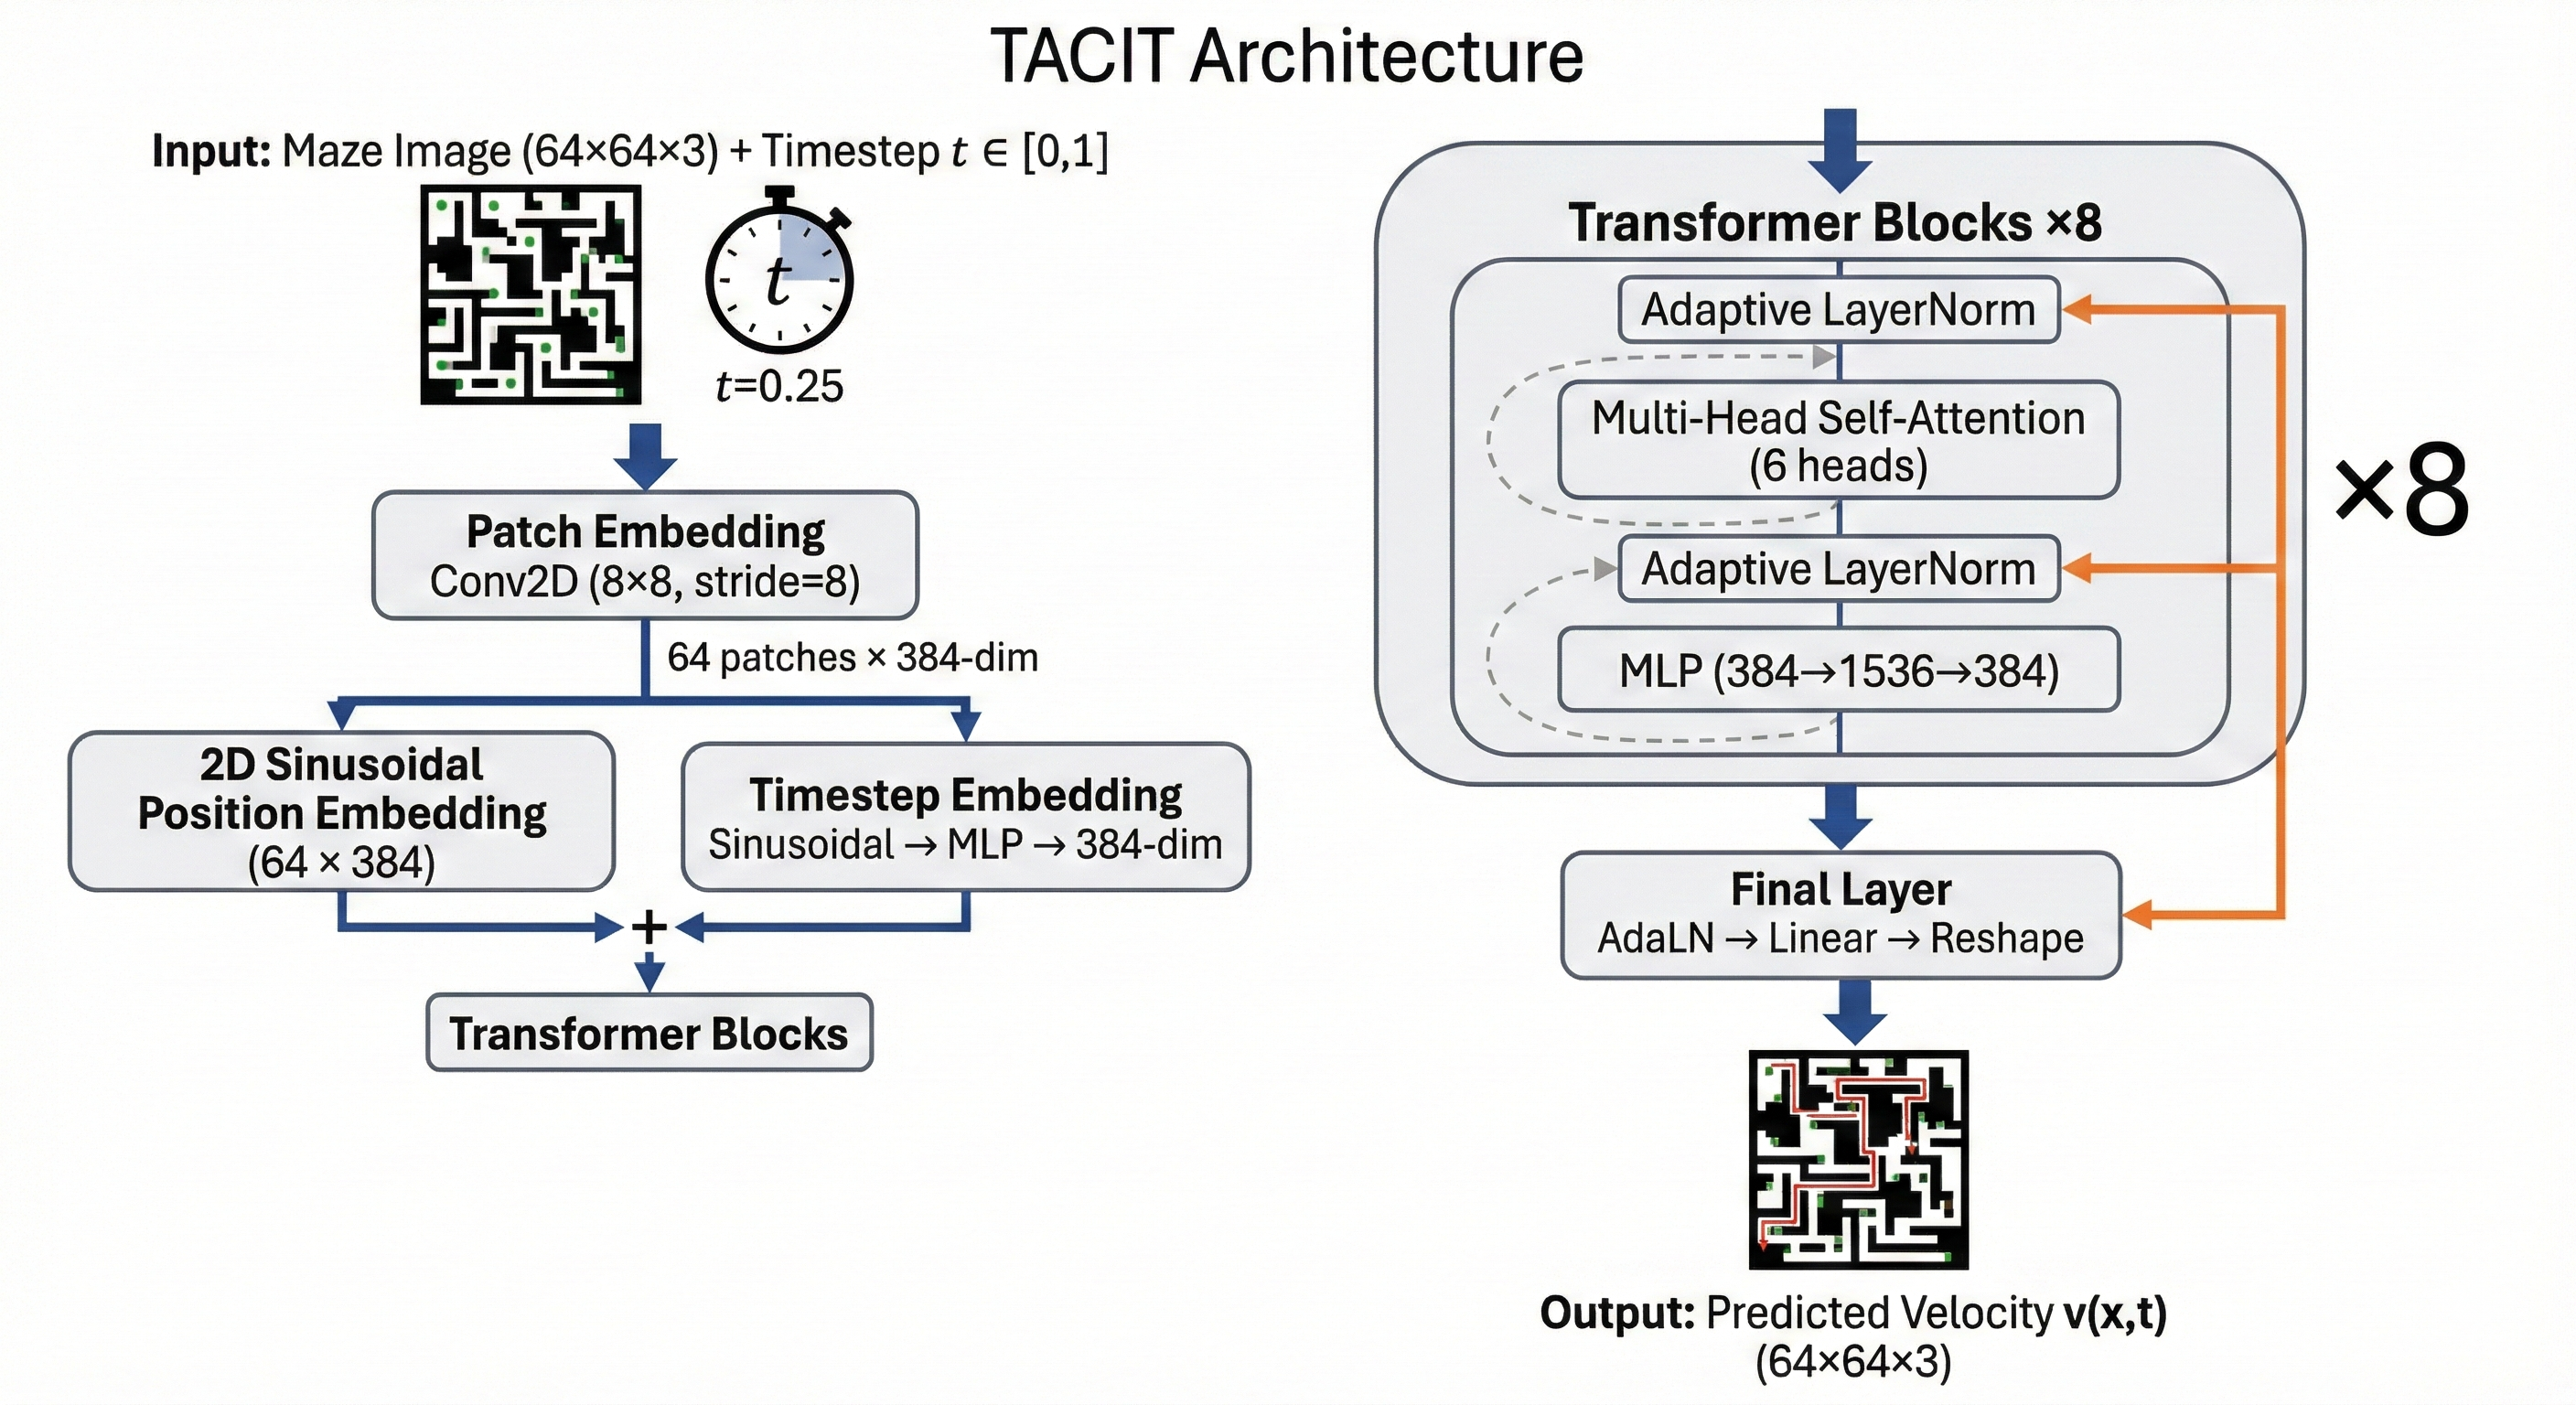
\includegraphics[width=0.9\textwidth]{architecture_diagram.pdf}
% \caption{TACIT architecture overview. Input images are tokenized into patches, processed through 8 transformer blocks with adaptive layer normalization, and reconstructed back to pixel space.}
% \label{fig:architecture}
% \end{figure}

\subsubsection{Patch Embedding}

Input images of size $64 \times 64 \times 3$ are divided into non-overlapping $8 \times 8$ patches, resulting in 64 patch tokens. Each patch is linearly projected to the hidden dimension:
\begin{equation}
    z_i = W_{\text{patch}} \cdot \text{flatten}(\text{patch}_i) + b_{\text{patch}}, \quad z_i \in \R^{384}
\end{equation}

The patch embedding is implemented as a 2D convolution with kernel size and stride equal to the patch size (8), effectively performing the flattening and projection in one operation.

\subsubsection{Positional Encoding}

We use 2D sinusoidal positional embeddings to encode spatial information. For each patch position $(p_x, p_y)$ on the $8 \times 8$ grid:
\begin{align}
    \text{PE}_{(p_x, p_y, 2i)} &= \sin\left(\frac{p_x}{10000^{2i/d}}\right) \\
    \text{PE}_{(p_x, p_y, 2i+1)} &= \cos\left(\frac{p_x}{10000^{2i/d}}\right)
\end{align}
with similar terms for $p_y$. The x and y embeddings are concatenated to form the full 384-dimensional position embedding, which is added to the patch embeddings.

\subsubsection{Timestep Embedding}

The diffusion timestep $t \in [0, 1]$ is encoded using sinusoidal embeddings followed by a two-layer MLP:
\begin{equation}
    e_t = \text{MLP}(\text{SinusoidalEmbed}(t)) \in \R^{384}
\end{equation}

The sinusoidal embedding uses 256 frequency components, providing multiple ``perspectives'' on the timestep at different temporal resolutions. The MLP consists of two linear layers (256 $\to$ 384 $\to$ 384) with SiLU activation.

\subsubsection{Transformer Blocks with Adaptive Layer Normalization}

The model consists of 8 transformer blocks. Each block uses \textit{adaptive layer normalization} (adaLN) to condition on the timestep embedding. Unlike standard layer normalization, adaLN learns to modulate the normalized activations based on the conditioning signal:
\begin{equation}
    \text{adaLN}(h, e_t) = \gamma(e_t) \odot \text{LayerNorm}(h) + \beta(e_t)
\end{equation}
where $\gamma$ and $\beta$ are predicted from the timestep embedding via a linear layer.

Each transformer block contains:
\begin{enumerate}
    \item \textbf{Adaptive LayerNorm 1}: Conditions the input before attention
    \item \textbf{Multi-Head Self-Attention}: 6 attention heads with head dimension 64
    \item \textbf{Residual connection}
    \item \textbf{Adaptive LayerNorm 2}: Conditions before the feedforward network
    \item \textbf{Feedforward Network}: Two-layer MLP (384 $\to$ 1536 $\to$ 384) with GELU activation
    \item \textbf{Residual connection}
\end{enumerate}

The self-attention mechanism allows each patch to attend to all other patches:
\begin{equation}
    \text{Attention}(Q, K, V) = \text{softmax}\left(\frac{QK^T}{\sqrt{d_k}}\right) V
\end{equation}
where $Q$, $K$, $V$ are linear projections of the input and $d_k = 64$ is the head dimension. We use PyTorch's \texttt{scaled\_dot\_product\_attention} which automatically selects efficient implementations (Flash Attention when available).

\subsubsection{Final Layer}

The final layer converts patch tokens back to image pixels:
\begin{enumerate}
    \item Adaptive layer normalization conditioned on timestep
    \item Linear projection: 384 $\to$ 192 (= $8 \times 8 \times 3$ pixels per patch)
    \item Reshape to image format: $(B, 64, 192) \to (B, 3, 64, 64)$
\end{enumerate}

\subsubsection{Architecture Summary}

Table~\ref{tab:architecture} summarizes the model hyperparameters.

\begin{table}[h]
\centering
\caption{Model architecture hyperparameters}
\label{tab:architecture}
\begin{tabular}{@{}ll@{}}
\toprule
\textbf{Component} & \textbf{Specification} \\
\midrule
Input resolution & $64 \times 64 \times 3$ \\
Patch size & $8 \times 8$ \\
Number of patches & 64 \\
Hidden dimension ($d$) & 384 \\
Transformer blocks & 8 \\
Attention heads & 6 \\
Head dimension & 64 \\
MLP hidden dimension & 1536 (4$\times d$) \\
Timestep embedding dimension & 256 \\
Total parameters & $\sim$50M \\
\bottomrule
\end{tabular}
\end{table}

\subsection{Inference via Euler Sampling}

At inference time, we integrate the learned velocity field using the Euler method:
\begin{equation}
    x_{t+\Delta t} = x_t + f_\theta(x_t, t) \cdot \Delta t
\end{equation}

Starting from $x_0$ (the unsolved maze), we take 10 Euler steps with $\Delta t = 0.1$ to arrive at the predicted solution $\hat{x}_1$. Algorithm~\ref{alg:euler} describes the sampling procedure.

\begin{algorithm}[h]
\caption{Euler Sampling for \tacit{}}
\label{alg:euler}
\begin{algorithmic}[1]
\REQUIRE Input image $x_0$, model $f_\theta$, number of steps $N=10$
\ENSURE Predicted solution $\hat{x}_1$
\STATE $x \leftarrow x_0$
\STATE $\Delta t \leftarrow 1/N$
\FOR{$i = 0$ to $N-1$}
    \STATE $t \leftarrow i \cdot \Delta t$
    \STATE $v \leftarrow f_\theta(x, t)$ \COMMENT{Predict velocity}
    \STATE $x \leftarrow x + v \cdot \Delta t$ \COMMENT{Euler step}
\ENDFOR
\RETURN $\text{clip}(x, 0, 1)$
\end{algorithmic}
\end{algorithm}

The deterministic nature of Euler sampling (no noise injection) means that each intermediate state $x_t$ is a meaningful interpolation that can be visualized. This is a key feature for interpretability: we can observe the model's ``reasoning trajectory'' from problem to solution.

%==============================================================================
\section{Dataset}
\label{sec:dataset}
%==============================================================================

\subsection{Maze Generation}

We generate mazes using a randomized depth-first search (DFS) algorithm with iterative backtracking:

\begin{enumerate}
    \item Initialize a grid where all cells are walls
    \item Start from position (1, 1), mark as path, push to stack
    \item While stack is non-empty:
    \begin{enumerate}
        \item Get unvisited neighbors (2 cells away to maintain wall structure)
        \item If neighbors exist: randomly choose one, carve path, push to stack
        \item Otherwise: backtrack (pop from stack)
    \end{enumerate}
\end{enumerate}

This generates perfect mazes (exactly one path between any two points) with varied complexity.

\subsection{Solution Finding}

Solutions are found using breadth-first search (BFS) from the top-left entry point (1, 1) to the bottom-right exit (size-2, size-2). BFS guarantees the shortest path, which is marked in red on the solved maze image.

\subsection{Image Rendering}

Mazes are rendered as $64 \times 64$ RGB images using nearest-neighbor interpolation to preserve sharp edges:
\begin{itemize}
    \item \textbf{White} (255, 255, 255): Path cells (traversable)
    \item \textbf{Black} (0, 0, 0): Wall cells
    \item \textbf{Green} (0, 255, 0): Entry and exit points
    \item \textbf{Red} (255, 0, 0): Solution path (target only)
\end{itemize}

\subsection{Dataset Statistics}

We generate diverse mazes with varying logical grid sizes:

\begin{table}[h]
\centering
\caption{Dataset characteristics}
\label{tab:dataset}
\begin{tabular}{@{}ll@{}}
\toprule
\textbf{Property} & \textbf{Value} \\
\midrule
Total pairs & 1,000,000 \\
Maze sizes (logical grid) & 11, 15, 21, 25, 31 \\
Image resolution & $64 \times 64$ \\
Channels & 3 (RGB) \\
Storage format & Compressed NumPy (.npz) \\
Batch file size & $\sim$120 MB (10,000 samples) \\
Total storage & $\sim$12 GB \\
\bottomrule
\end{tabular}
\end{table}

The varying maze sizes ensure the model learns to handle different complexity levels. Smaller mazes (11$\times$11) have shorter solutions, while larger mazes (31$\times$31) require longer, more complex paths.

\subsection{Data Loading}

We implement lazy batch loading for memory efficiency:
\begin{itemize}
    \item Dataset stored in 100 batch files (10,000 pairs each)
    \item Only one batch loaded in memory at a time
    \item Batch files shuffled each epoch
    \item Samples shuffled within each batch
    \item Multi-worker loading (8 workers) with prefetching
\end{itemize}

%==============================================================================
\section{Experiments}
\label{sec:experiments}
%==============================================================================

\subsection{Training Configuration}

We train \tacit{} with the following configuration:

\begin{table}[h]
\centering
\caption{Training hyperparameters}
\label{tab:training}
\begin{tabular}{@{}ll@{}}
\toprule
\textbf{Parameter} & \textbf{Value} \\
\midrule
Optimizer & Adam \\
Learning rate & $1 \times 10^{-4}$ \\
Batch size & 256 \\
Total epochs & 100 \\
Mixed precision & Enabled (FP16 with gradient scaling) \\
Model compilation & torch.compile() \\
Checkpoint interval & Every 5 epochs \\
\bottomrule
\end{tabular}
\end{table}

Training uses automatic mixed precision (AMP) for efficiency and \texttt{torch.compile()} for graph-level optimization. The model is trained on NVIDIA A100 GPU.

\subsection{Training Dynamics}

\begin{figure}[t]
\centering
\includegraphics[width=0.8\textwidth]{training_curves/loss_curve_log.png}
\caption{Training loss over 100 epochs (log scale). The model exhibits three phases: rapid learning (epochs 1-25), refinement (epochs 25-60), and fine-tuning (epochs 60-100). Total loss reduction: 192$\times$ from epoch 5 to epoch 100.}
\label{fig:loss_curve}
\end{figure}

Figure~\ref{fig:loss_curve} shows the training loss over 100 epochs. We observe three distinct phases:

\paragraph{Phase 1: Rapid Learning (Epochs 1-25).}
Loss decreases from $1.2 \times 10^{-3}$ to $4.0 \times 10^{-5}$ (30$\times$ reduction). The model learns basic maze structure and begins producing recognizable outputs.

\paragraph{Phase 2: Refinement (Epochs 25-60).}
Loss continues decreasing to approximately $1.1 \times 10^{-5}$ (additional 3.6$\times$ reduction). Visual quality improves with cleaner paths and fewer artifacts.

\paragraph{Phase 3: Fine-tuning (Epochs 60-100).}
Loss converges to $6.25 \times 10^{-6}$ (additional 1.8$\times$ reduction). The model produces high-quality solutions with minimal artifacts.

\begin{table}[h]
\centering
\caption{Training loss progression}
\label{tab:loss}
\begin{tabular}{@{}ccc@{}}
\toprule
\textbf{Epoch} & \textbf{Loss} & \textbf{Improvement vs Epoch 5} \\
\midrule
5 & $1.20 \times 10^{-3}$ & --- \\
10 & $3.50 \times 10^{-4}$ & 3.4$\times$ \\
25 & $4.00 \times 10^{-5}$ & 30$\times$ \\
50 & $1.31 \times 10^{-5}$ & 92$\times$ \\
75 & $8.81 \times 10^{-6}$ & 136$\times$ \\
100 & $6.25 \times 10^{-6}$ & 192$\times$ \\
\bottomrule
\end{tabular}
\end{table}

\subsection{Prediction Quality}

\begin{figure}[t]
\centering
\includegraphics[width=0.8\textwidth]{training_curves/quality_metrics.png}
\caption{Prediction quality measured as L2 distance to ground truth over training epochs. Lower values indicate better predictions. The model achieves 22.7$\times$ improvement from epoch 5 to epoch 100.}
\label{fig:quality}
\end{figure}

We evaluate prediction quality using L2 distance (MSE) between the model's output and the ground truth solution, measured on held-out samples at each checkpoint (Figure~\ref{fig:quality}).

\begin{table}[h]
\centering
\caption{Prediction quality (L2 distance to ground truth)}
\label{tab:quality}
\begin{tabular}{@{}ccc@{}}
\toprule
\textbf{Epoch} & \textbf{Avg L2 Distance} & \textbf{Improvement vs Epoch 5} \\
\midrule
5 & 0.0318 & --- \\
10 & 0.0191 & 1.7$\times$ \\
25 & 0.0071 & 4.5$\times$ \\
50 & 0.0053 & 6.0$\times$ \\
75 & 0.0060 & 5.3$\times$ \\
100 & 0.0014 & 22.7$\times$ \\
\bottomrule
\end{tabular}
\end{table}

The final model achieves an L2 distance of 0.0014, representing a 22.7$\times$ improvement over the epoch 5 baseline. Some variance is observed (e.g., epoch 75 has slightly higher L2 than epoch 70), which we attribute to the stochastic nature of evaluation sampling.

\subsection{Training Throughput}

Training achieves an average throughput of approximately 7,000 samples per second, with peak throughput of 11,700 samples/second during epochs 45-60. This corresponds to approximately 4 hours of total training time. The throughput increase during mid-training is likely due to accumulated benefits from \texttt{torch.compile()} kernel fusion.

\subsection{Qualitative Results}

\begin{figure}[t]
\centering
\includegraphics[width=\textwidth]{epoch_comparison/evolution_grid.png}
\caption{Visual evolution of model outputs across training. Each row shows a different maze sample. Columns show model predictions at epochs 5, 10, 25, 50, 75, and 100 (left to right). Early epochs produce blurry outputs, while later epochs produce accurate solutions with the correct path marked in red.}
\label{fig:evolution}
\end{figure}

Visual inspection of model outputs across training reveals a clear progression (Figure~\ref{fig:evolution}):

\begin{itemize}
    \item \textbf{Epoch 5}: Outputs are blurry with no discernible path structure
    \item \textbf{Epoch 10}: Basic maze structure emerges, but paths are incomplete and noisy
    \item \textbf{Epoch 25}: Clear walls and paths, solutions begin to appear but may be incomplete
    \item \textbf{Epoch 50}: Good quality solutions, occasional minor artifacts
    \item \textbf{Epoch 75}: High quality outputs, rare errors
    \item \textbf{Epoch 100}: Excellent quality, accurate solutions with minimal artifacts
\end{itemize}

%==============================================================================
\section{Interpretability Analysis}
\label{sec:interpretability}
%==============================================================================

A central motivation for \tacit{}'s design is interpretability. By operating in pixel space with rectified flow and deterministic Euler sampling, we can visualize the model's reasoning process as it transforms an unsolved maze into a solution.

\subsection{Inference Trajectory Visualization}

During inference, we record intermediate states at each of the 10 Euler steps. These states represent the model's progressive transformation from input ($t=0$) to output ($t=1$). Unlike DDPM-style diffusion where intermediate states are corrupted by noise, our intermediate states are clean images that can be directly interpreted.

Qualitative observation of these trajectories reveals:
\begin{itemize}
    \item \textbf{Early steps} ($t < 0.3$): The model begins to ``highlight'' potential path regions
    \item \textbf{Middle steps} ($0.3 < t < 0.7$): Solution path emerges progressively, often starting from entry/exit points
    \item \textbf{Late steps} ($t > 0.7$): Refinement of path color intensity and removal of artifacts
\end{itemize}

This step-by-step visualization provides insight into the model's implicit reasoning strategy---whether it constructs the solution incrementally from endpoints, globally, or through some other mechanism.

\subsection{Design Decisions for Interpretability}

Several design choices specifically enable this interpretability:

\paragraph{Pixel Space vs. Latent Space.}
Operating directly on pixels rather than VAE latents ensures that:
\begin{enumerate}
    \item Intermediate states are actual images, not abstract vectors
    \item Discrete structural information (wall/path boundaries) is preserved
    \item No additional decoder is needed to visualize internal states
\end{enumerate}

\paragraph{Rectified Flow vs. DDPM.}
Standard diffusion adds Gaussian noise during training and inference. With rectified flow:
\begin{enumerate}
    \item Interpolated training states $x_t$ are clean blends of input and output
    \item Inference follows deterministic paths without stochastic noise
    \item The same input always produces the same trajectory
\end{enumerate}

\paragraph{Euler Sampling.}
Simple Euler integration with 10 steps provides:
\begin{enumerate}
    \item Discrete, observable intermediate states
    \item Direct correspondence between step number and ``progress'' toward solution
    \item Computational efficiency (only 10 forward passes)
\end{enumerate}

%==============================================================================
\section{Discussion}
\label{sec:discussion}
%==============================================================================

\subsection{Tacit Knowledge in Neural Networks}

The name ``TACIT'' references the concept of tacit knowledge---knowledge that is difficult to articulate explicitly but guides behavior effectively. Expert chess players, for instance, often cannot fully explain their intuitions about board positions, yet reliably make strong moves.

Our model demonstrates a similar phenomenon: it learns to solve mazes without explicit programming of search algorithms (BFS, DFS, A*). The ``reasoning'' emerges from the statistical patterns in the training data, encoded in the network's weights. The flow matching formulation captures this as a continuous transformation from problem to solution state.

\subsection{Language-Free Visual Reasoning}

Contemporary AI reasoning systems often rely heavily on language. Chain-of-thought prompting, reasoning tokens, and scratchpad methods all externalize reasoning through text. While effective, this approach:
\begin{enumerate}
    \item Ties reasoning to linguistic representation
    \item May not capture visual-spatial intuitions well
    \item Requires language as an intermediary
\end{enumerate}

\tacit{} explores whether reasoning can emerge from purely visual supervision. The model receives only image pairs (problem, solution) and learns the transformation between them. This represents a different paradigm---one closer to how biological visual systems might develop intuitions through experience rather than explicit instruction.

\subsection{Relationship to World Models}

World models aim to learn internal representations of environment dynamics that support prediction and planning. \tacit{} can be viewed as learning a ``world model'' for the maze domain:
\begin{itemize}
    \item The model implicitly represents maze topology (walls, paths, connectivity)
    \item The flow encodes the transformation from problem to solution state
    \item Intermediate states may encode partial planning or search
\end{itemize}

Unlike JEPA-style approaches that operate in abstract latent spaces, our pixel-space design prioritizes interpretability over representational efficiency.

\subsection{Limitations}

\paragraph{Domain Specificity.}
The current model is trained only on mazes. Generalization to other visual reasoning tasks (abstract pattern recognition, spatial transformations) requires additional investigation.

\paragraph{Evaluation Metrics.}
While L2 distance captures pixel-level accuracy, it may not fully reflect solution validity. Future work should incorporate path verification metrics (connectivity, correctness).

\paragraph{Scale.}
The $64 \times 64$ resolution and relatively small model (50M parameters) limit complexity. Scaling to larger images and models may reveal additional capabilities or limitations.

\subsection{Future Directions}

\paragraph{Bidirectional Flow.}
Training the reverse direction (solution $\to$ problem) would test whether the model learns genuine bidirectional understanding rather than unidirectional mapping.

\paragraph{Probing Internal Representations.}
Analyzing activations at different transformer blocks could reveal hierarchical reasoning---e.g., early blocks detecting local features, later blocks integrating global path information.

\paragraph{Generalization Studies.}
Testing on out-of-distribution mazes (larger sizes, different generation algorithms, obstacles) would characterize the model's reasoning generalization.

\paragraph{Alternative Domains.}
Applying the approach to other visual reasoning benchmarks (RAVEN, ARC) would test the generality of flow matching for reasoning tasks.

%==============================================================================
\section{Conclusion}
\label{sec:conclusion}
%==============================================================================

We presented \tacit{}, a diffusion-based transformer for interpretable visual reasoning. By combining flow matching with pixel-space operation and deterministic Euler sampling, we create a system where reasoning can be directly observed as a continuous transformation from problem to solution.

Trained on 1 million maze-solving examples, the model achieves strong performance (192$\times$ loss reduction, 22.7$\times$ improvement in L2 distance) while producing interpretable intermediate states during inference. The design prioritizes understanding over performance, establishing a foundation for studying how neural networks develop and apply implicit reasoning strategies.

The broader implication is that language may not be necessary for reasoning---at least for certain visual-spatial domains. By learning transformations between visual states, models can capture structural relationships and problem-solving strategies in a fundamentally different way than language-based approaches. This opens new directions for understanding and building AI systems with genuine visual reasoning capabilities.

%==============================================================================
\section*{Reproducibility}
%==============================================================================

All code, model weights, and datasets are publicly available:
\begin{itemize}
    \item Code: \url{https://github.com/danielxmed/tacit}
    \item Model: \url{https://huggingface.co/tylerxdurden/tacit}
    \item Dataset: \url{https://huggingface.co/datasets/tylerxdurden/maze}
\end{itemize}

Training was performed on NVIDIA A100 GPU with PyTorch 2.0+. Checkpoints are saved in SafeTensors format at 5-epoch intervals. The complete training pipeline can be reproduced using the provided scripts.

%==============================================================================
% Placeholder for references - to be added later
%==============================================================================

\section*{References}

\textit{[References to be added in final version]}

\begin{itemize}
    \item Liu et al. (2022) - Rectified Flow / Flow Matching
    \item Peebles \& Xie (2023) - Scalable Diffusion Models with Transformers (DiT)
    \item Dosovitskiy et al. (2020) - Vision Transformer (ViT)
    \item Ho et al. (2020) - Denoising Diffusion Probabilistic Models
    \item Polanyi (1966) - The Tacit Dimension
    \item LeCun (2022) - A Path Towards Autonomous Machine Intelligence (JEPA)
    \item RAVEN, PGM, ARC benchmarks
\end{itemize}

\end{document}
